% An exact map of four equally likely elementary outcomes to three unequal masses.
% All probabilities come from the four ordered outcomes of two independent fair tosses.
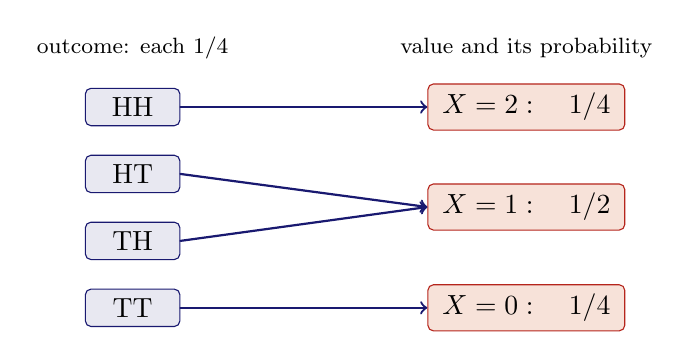
\begin{tikzpicture}[x=1cm,y=1cm,line cap=round]
  \node[font=\footnotesize] at (0,3.55) {outcome: each $1/4$};
  \node[font=\footnotesize] at (5.0,3.55) {value and its probability};
  \node[draw=MidnightBlue,fill=MidnightBlue!10,rounded corners=2pt,minimum width=1.2cm] (hh) at (0,2.8) {HH};
  \node[draw=MidnightBlue,fill=MidnightBlue!10,rounded corners=2pt,minimum width=1.2cm] (ht) at (0,1.95) {HT};
  \node[draw=MidnightBlue,fill=MidnightBlue!10,rounded corners=2pt,minimum width=1.2cm] (th) at (0,1.10) {TH};
  \node[draw=MidnightBlue,fill=MidnightBlue!10,rounded corners=2pt,minimum width=1.2cm] (tt) at (0,0.25) {TT};
  \node[draw=BrickRed,fill=BrickRed!10,rounded corners=2pt,minimum width=2.5cm] (two) at (5,2.8) {$X=2:\quad 1/4$};
  \node[draw=BrickRed,fill=BrickRed!10,rounded corners=2pt,minimum width=2.5cm] (one) at (5,1.53) {$X=1:\quad 1/2$};
  \node[draw=BrickRed,fill=BrickRed!10,rounded corners=2pt,minimum width=2.5cm] (zero) at (5,0.25) {$X=0:\quad 1/4$};
  \draw[->,MidnightBlue,thick] (hh.east)--(two.west);
  \draw[->,MidnightBlue,thick] (ht.east)--(one.west);
  \draw[->,MidnightBlue,thick] (th.east)--(one.west);
  \draw[->,MidnightBlue,thick] (tt.east)--(zero.west);
\end{tikzpicture}
